\documentclass[a4paper,10pt]{article}
\usepackage[a4paper,vmargin={10mm,20mm},hmargin={20mm,20mm}]{geometry}
\usepackage{cmap}
\usepackage[utf8]{inputenc}
\usepackage[T1]{fontenc}
\usepackage{lmodern}
\usepackage[ngerman]{babel}
\usepackage[babel=true]{microtype}
\usepackage{enumitem}
\setlist{nolistsep}
\usepackage{graphicx}
\usepackage{color,soul}
\usepackage[usenames,dvipsnames]{xcolor}
\usepackage[pdfborder={0 0 0}]{hyperref}
\input glyphtounicode
\pdfgentounicode=1
\parindent 0cm
\parskip1.5ex plus0.5ex minus0.5ex
% \usepackage{titling}
% \setlength{\droptitle}{-4em}     % Eliminate the default vertical space
% \addtolength{\droptitle}{-100pt}   % Only a guess. Use this for adjustment
\pagenumbering{gobble}

\newcommand{\colloc}[1]{\sethlcolor{red}\hl{#1}}
\newcommand{\colhop}[1]{\sethlcolor{yellow}\hl{#1}}
\newcommand{\colrem}[1]{\sethlcolor{green}\hl{#1}}

\title{SSH Tunnel / Local Port Forwarding}
\author{Michael Nagel\\\href{mailto:michael.nagel@devzero.de}{michael.nagel@devzero.de}}
\date{10. Mai 2013}

\pdfinfo{%
  /Title    (SSH Tunnel / Local Port Forwarding)
  /Author   (Michael Nagel)
  /Subject  (SSH Tunnel / Local Port Forwarding)
  /Keywords (SSH Tunnel / Local Port Forwarding)
}

\setlength{\marginparwidth}{20mm}

\begin{document}
\maketitle

„HILFE!!! Ich möchte von meinem Laptop auf einen MySQL-Server zugreifen, der aus Sicherheitsgründen nur lokale Verbindungen zulässt!!!“ \textit{Typischer Hilfeschrei}

Jemand möchte von \colloc{seinem Rechner} auf einen \colrem{bestimmten Port} auf \colrem{einem Server} zugreifen.
Eine Firewall blockiert den direkten Zugriff.
Ein \colhop{weiterer Rechner}, der per SSH erreichbar ist, hat jedoch Zugriff auf \colrem{den Port} auf \colrem{dem Server}.

\begin{large}
\begin{center}
\textbf{Lösung: SSH Tunnel / Local Port Forwarding}
\end{center}
\end{large}

Lokales SSH Port Forwarding erlaubt es (unter anderem) über einen sogenannten \colhop{Hopping Host} Zugriff auf \colrem{einen Server} hinter einer Firewall zu erhalten.

Folgende Angaben sind dazu erforderlich:
\begin{itemize}
 \item  \colloc{lokaler Host und lokaler Port} – lokaler Host ist dort, wo SSH/putty läuft
 \item \colhop{Hopping Host}
 \item \colrem{Ziel-Host} (aus Sicht von \colhop{Hopping Host (localhost)}) und \colrem{Ziel-Port}
\end{itemize}



Beispiel: Jemand möchte von  \colloc{seinem Laptop} aus auf eine Datenbank auf example.de zugreifen. Er hat SSH-Zugriff auf \colhop{example.de}.

Mit OpenSSH (Mac, Linux) sieht der Aufruf zur Tunnel-Erstellung folgendermaßen aus:

\texttt{\$ ssh \colhop{login@example.de} -L \colloc{9999}:\colrem{localhost}:\colrem{3306}}

Solange das Port-Forwarding aktiv ist, kommen Daten, die an „\colloc{lokaler Host:lokaler Port}“ gesendet werden, bei „\colrem{Ziel-Host:Ziel-Port}“ an.
Statt „mysql -h \colrem{example.de} -P \colrem{3306}“ kann jetzt „mysql -h  \colloc{localhost} -P  \colloc{9999}“ verwendet werden,
um sich mit dem Datenbank-Server zu verbinden und die Daten erreichen über den Tunnel ihr bislang unerreichbares Ziel.

Unter Windows mit PuTTY sind bei einer \colhop{example.de}-Session die folgenden Einstellungen nötig:

\begin{figure}[ht!]
 \centering
 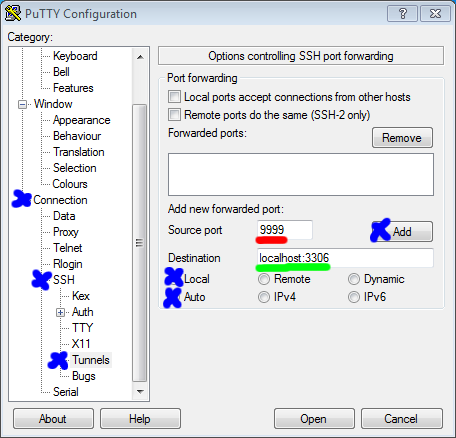
\includegraphics[width=200pt,height=200pt]{./putty-create-tunnel.png}
 \caption{PuTTY Tunnel-Einstellungen}
 \label{fig:putty}
\end{figure}


\end{document}
